\chapter{JSIM\emph{wiz}}
\label{cha:jsimwiz}
\section{Overview}
Simulation technique can be applied when the characteristics of
the network to be analyzed make the analytical techniques no
longer useful for its performance evaluation. A simulator is a
dynamic model able to follow the evolution in time of either the
system complexity it represents and the pattern of arrival
requests to be executed.\\
In the JMT \emph{suite} a discrete-event simulator JSIM for the
analysis of queueing network models is provided. It can be used
through two interfaces: alphanumerical (JSIM\emph{wiz}) and
graphical (JSIM\emph{graph}). \textbf{The manual of
JSIM\emph{graph} follows this one, and should be consulted if some
information are omitted or unclear in the present manual.}

An intuitive user interface allows even an unexperienced user to
build with JSIM\emph{wiz} system models with sophisticated
characteristics. It helps the users to perform an evaluation study
in two ways. Firstly, critical statistical decisions, such as
transient detection and removal, variance estimation, and
simulation length control, have been \emph{completely automated},
thus freeing the users from taking decisions about parameters s/he
may not be familiar with. The simulation is automatically stopped
when all performance indexes can be estimated with the required
accuracy. Secondly, a user-friendly graphical interface allows the
user to describe, both the network layout and the input
parameters. Furthermore, the graphical interface also provides
support for the use of advanced features (several of them are for
networks with very general characteristics, usually referred to as
\emph{non-product-form} networks) like fork and join of customers,
blocking mechanisms, regions with capacity constraints on
population, state-dependent routing strategies, user-defined
general distributions, import and reuse of log data. A module for
\emph{What-If Analysis}, where a sequence of simulations is run
for different values of control parameters, particularly useful in
capacity planning, tuning and optimization studies, is also
provided.

The simulation engine performs on-line the statistical analysis of
measured performance indices, plots the collected values, discards
the initial
transient periods and computes the confidence intervals.\\
All the plots generated by a simulation can be exported in vector
(e.g., eps, pdf) or raster (e.g., jpeg,
png) image formats.\\

\ \\
\noindent \textbf{\large Main Features}\\
\noindent \textbf{Arrival rates} for open classes of customers
generated by Source stations and station \emph{service times} (for
any type of station in open and closed models) can be generated
according to the following distributions: Burst (general),
Constant, Erlang, Exponential, Gamma, Hyperexponential, Normal,
Pareto, Poisson,
Student-T, Uniform \\

\noindent \textbf{Queueing discipline}: the following strategies
are available:  First Come First Served, FCFS with priority, Last
Come First Served, LCFS with priority\\

\noindent \textbf{Routing} of the customers in the network, i.e.,
the path followed by the requests among the resources, can be
described either probabilistically or according to the following
strategies: Fastest service, Least utilization, Random, Round
robin, Join the Shortest Queue, Shortest response time (the values
of the control parameters are evaluated on the stations connected
in output to the considered one). These strategies can be further
combined among themselves through the use of a \emph{routing
station}.\\

\noindent \textbf{Other peculiar features} of the simulator are:
\vspace{-0.2cm}
\begin{itemize*}
    \item Load dependent service time strategies
    \item Fork-and-join stations to model parallelism
    \item Simulation of complex traffic pattern and service times (e.g., burst)
    \item Blocking regions (in which the number of customer is limited)
    \item What-if analysis (with various control parameters)
    \item Customization of default values
    \item Import/Export of the model from/to JMVA, the exact solver (when
    the required analytic assumptions are satisfied)
    \item Logging of the data flowing in any part of the model
    (\emph{Logger} station)
    \item Graphical visualization of the evaluated performance
    indices together with their confidence intervals
    \item automatic transient detection and removal
    \item automatic stop of the simulation when all performance
    metrics can be estimated with the required accuracy.
\end{itemize*}
JSIM\emph{wiz} has a modular Java-based architecture that allows
the introduction of new Java classes in the simulation engine
without any modification to the source codes of the other classes.


\subsection{Starting the discrete-event simulator}
Selecting 
\includegraphics[scale=.5]{img/JSIMIcon.eps} button on the
starting screen, \autoref{fig:jsim:Classes} window shows up.
\begin{figure}[htb]
    \begin{center}
        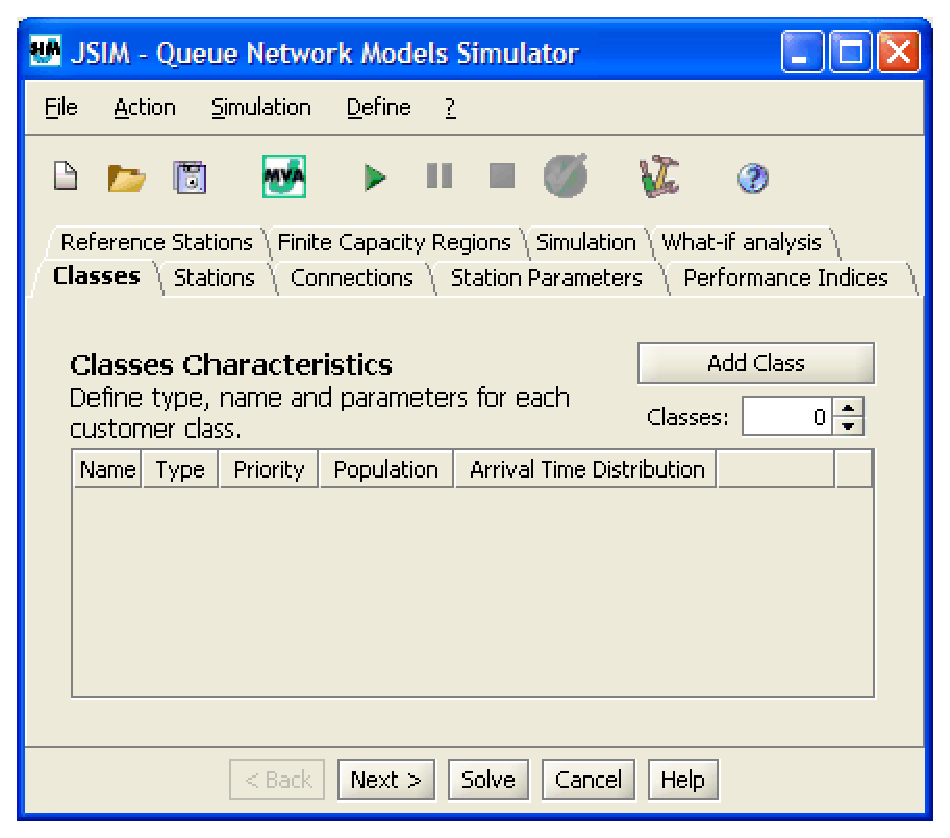
\includegraphics[scale=.5]{img/jsim/define_class1.eps}
    \end{center}
    \caption{The home window of JSIM\emph{wiz} simulator}
    \label{fig:jsim:Classes}
\end{figure}
Three main areas are shown:
\begin{description*}
\item[Menu :] it is organized into three groups of functions. To use a
menu, click on the menu heading and choose the appropriate option.
For the description of menu entries, see \autoref{sec:jmva:Menu}
\item[Toolbar :] contains some buttons to speed up access to JSIM functions
(e.g. New model, Open, Save\dots ). If you move the mouse pointer over a button a tooltip will be shown up.
\item[Page Area :] this is the core of the window. All JSIM parameters are grouped in
different tabs. You can modify only a subset of them by selecting
the right tab, as will be shown later.
\end{description*}

\section{Defining a new model}
\label{sec:DefiningANewModel}
To define a new model, select the New command from the File menu, or the button 
\includegraphics[scale=.5]{img/jsim/new.eps} or use the shortcut CTRL+N. A new model is automatically created every time JSIM is started.\\\\
The following parameters must be defined in order to complete the new model:
\begin{itemize*}
\item Classes
\item Stations
\item Connections
\item Station parameters \textbf{*}
\item Performance indices
\item Reference stations
\item Finite capacity regions \textbf{*}
\item Simulation *
\end{itemize*}
To set each parameter, follow the user manual step by step.

\noindent \textbf{NOTE:} if no values are provided for the parameters marked with \textbf{*}, default values will be used and the simulation will run anyway.

\subsection{Define Classes}
\label{sec:DefineClasses}
Customer classes identify different customer behavior and characteristics, such as the type (closed or open), the size of the customer population (for closed classes) or the interarrival time distribution (for open classes).
They can be set using the \textbf{Classes} tab during the creation of a new model.\\
\begin{center}
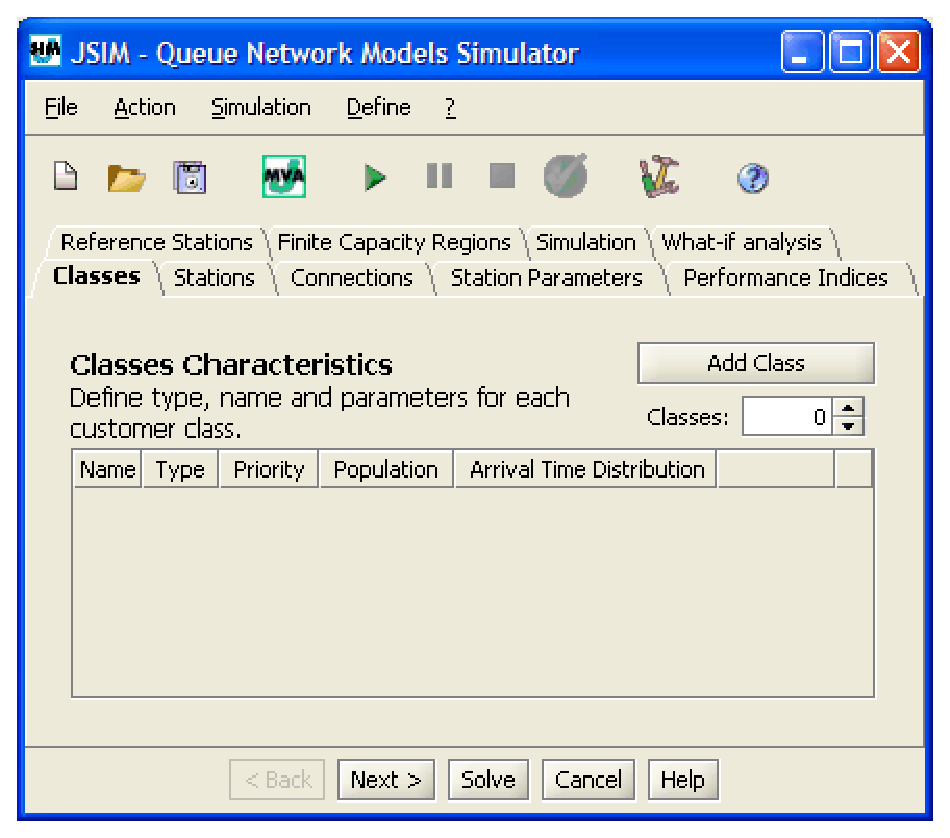
\includegraphics[scale=.5]{img/jsim/define_class1}
\end{center}

\noindent\textbf{\large{Adding a Class}}

Classes must be explicitly added to the model, either one at a time by clicking the 
\includegraphics[scale=.5]{img/jsim/button_addClass.eps} button, or by selecting directly the final number of classes desired in the form 
\includegraphics[scale=.5]{img/jsim/button_NClass.eps}. The newly added classes will be listed with deafult parameters.\\
Double click on the default name (ClassN) to change it.\\
Each new class has a priority in the system. A smaller number indicates a lower priority. Default value is 0 and it can be changed by double clicking on the corresponding area.\\\\
\textbf{\large{Defining the Class Type: Open Classes}}

After adding a class and possibly changing its name and priority, you must choose the type of customers comprising the class. Classes are created Closed by default, so if you want an Open class, select the type Open in the menu\\
\begin{figure}
\begin{center}

\includegraphics[scale=.5]{img/jsim/type_class.eps}
\end{center}
\end{figure}

The class characteristics looks like this now
\begin{figure}
\begin{center}
%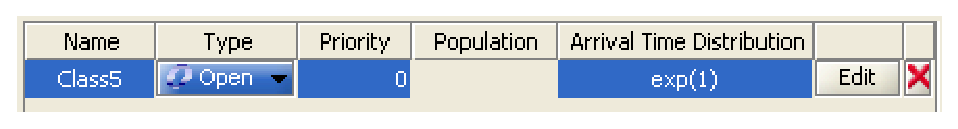
\includegraphics[scale=.5]{img/jsim/open_class1.eps}
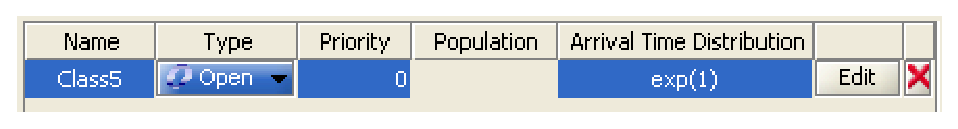
\includegraphics[scale=.5]{img/jsim/open_class1.eps}

\end{center}
\end{figure}

Open classes describe customer populations that vary during time,
therefore they are best characterized by the probability
distribution of the interarrival time, rather than by a constant
number of customers. The default Interarrival Time Distribution is
exp(1) (Exponential Distribution with $\lambda$ =1).\\ To change
the Interarrival Time Distribution click the Edit button
\begin{center}

\includegraphics[scale=.5]{img/jsim/arrival_time_distribution1.eps}
\end{center}

The following window will appear
\begin{center}
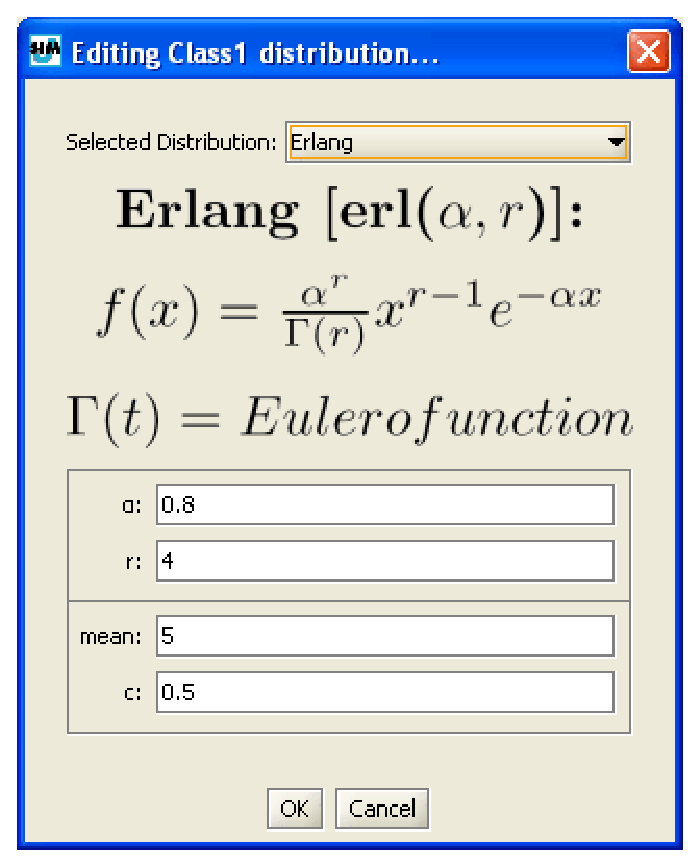
\includegraphics[scale=.5]{img/jsim/erlang.eps}
\end{center}

Click on the Selected Distribution drop down menu to choose from any of the following
distributions \autoref{sec:Distributions}:
\begin{itemize*}
    \item Burst
    \item Constant
    \item Erlang
    \item Exponential
    \item Gamma
    \item Hyperexponential
    \item Normal
    \item Pareto
    \item Poisson
    \item Replayer
    \item StudentT
    \item Uniform
\end{itemize*}

In each case, it is possible to configure the distribution parameters as you wish, or use the default values. Parameters that are related among each other are automatically adjusted if one is modified (for example,the figure shows how for an Erlang distribution, if you set the (alfa, r) pair, the (mean, c) pair is automatically adjusted to the correct value).
The Replayer distribution allows you to provide data traces from files.
Click OK when you are done to return to Class parameters definition.\\
The final step in defining a class is the definition of the Reference Station, i.e., that station in the model with respect to which the performance indices will be computed. For Open classes there is no choice since the Source station is the unchangeable default Reference Station used to compute System Throughput for all the Open classes.\\
\begin{center}
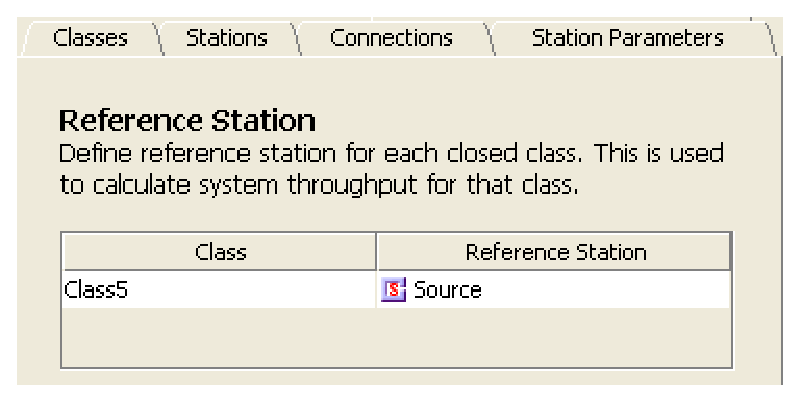
\includegraphics[scale=.5]{img/jsim/reference_open1.eps}
\end{center}

\textbf{\large{Defining the Class Type: Closed Classes}}\\
\begin{center}

\includegraphics[scale=.5]{img/jsim/closed_class1.eps}
\end{center}

Classes are created Closed by default, so there is not need to change the Type. Priority can be changed as in the Open class case. The population size is the parameter that characterizes a Closed class. It is fixed and does not change for the entire life of the system. By default is 1 and it can be changed by clicking on the corresponding area in the class properties matrix.\\\\
The final step is to define a Reference Station for the class that will be used to compute the performance indices selected for the class. Use the Reference Station tab menu to select the Station.All stations but the sink can be used as reference station for a closed class.\\
\begin{center}
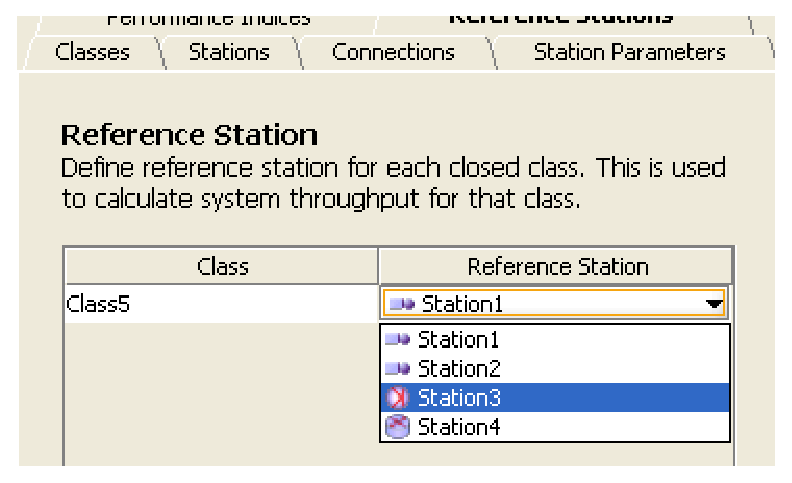
\includegraphics[scale=.5]{img/jsim/reference_closed1.eps}
\end{center}

\subsubsection{Distributions}
\label{sec:Distributions}

Open classes model transaction workloads where the number of requests in the system fluctuates over time and transactions arrive at the system as if generated by an infinite source. The arrival pattern is well described by a probability distribution, in particular, the distribution of the interarrival times of consecutive transactions, or \emph{customers}.
A probability distribution f(x) is characterized by :
\begin{itemize*}
\item Mean (if exists): 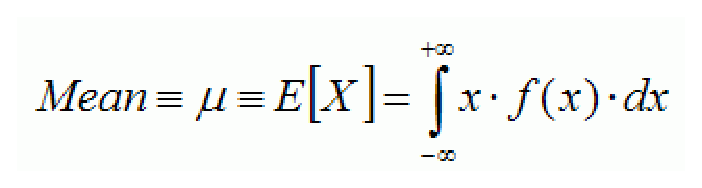
\includegraphics[scale=.5]{img/jsim/Mean.eps}
\item Variance (if exists): 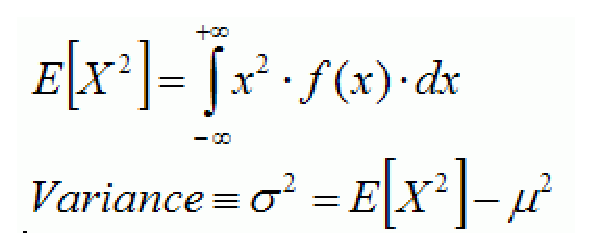
\includegraphics[scale=.5]{img/jsim/variance.eps}
\item c, Coefficient of Variation, only if mean and variance exist and mean is not zero: 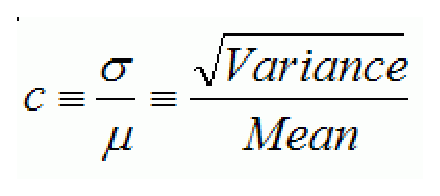
\includegraphics[scale=.5]{img/jsim/CoeffVariation.eps}
\end{itemize*}
JSIM\emph{wiz} allows you to use any of the following probability distributions:
\\ % DISTR %
\textbf{Constant: }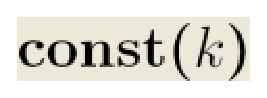
\includegraphics[scale=.5]{img/jsim/constant_f.eps}
\\\\
\noindent Probability density function:
\begin{center}
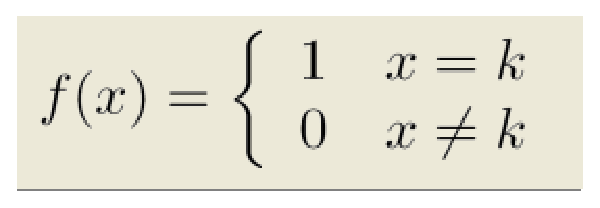
\includegraphics[scale=.5]{img/jsim/constant1.eps}
\end{center}

The mean is equal to \emph{k}, which is the parameter  you must specify.
This distribution describes a constant flow of customers, arriving exactly every \emph{k} time units.\\
\begin{center}
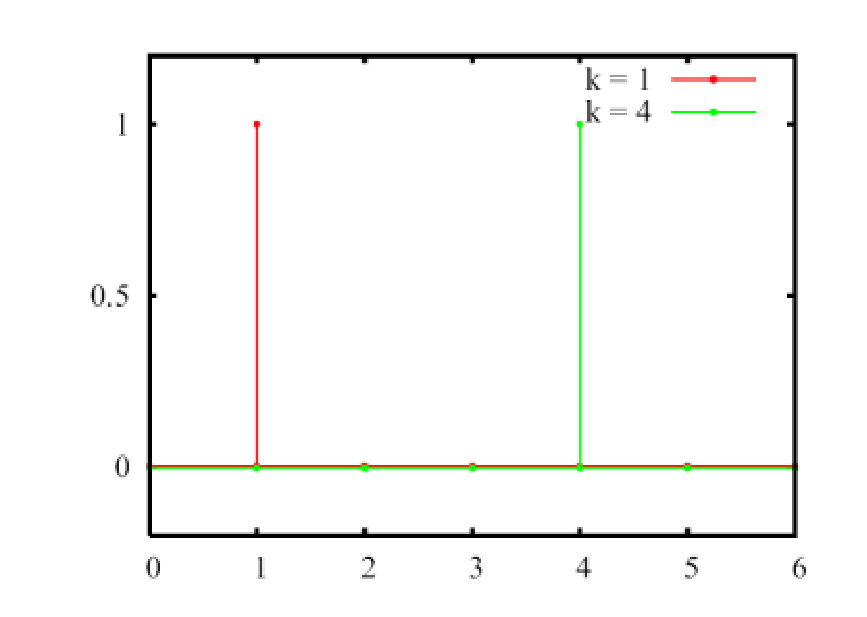
\includegraphics[scale=.5]{img/jsim/const_pdf.eps}
\end{center}


% DISTR %
\textbf{Erlang:}
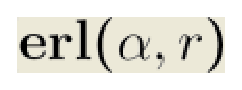
\includegraphics[scale=.5]{img/jsim/erlang_f.eps}
\\ \\
Probability density function
\\\\
The Erlang distribution is a continuous distribution, with 2 parameters: the \emph{shape r}, an integer value, and the rate \emph{$\alpha$}, a real value. It is a special case of Gamma distribution where the shape parameter is an integer.
\\
$\Gamma (t)$ is called Eulero function and is defined by \\
\begin{center}
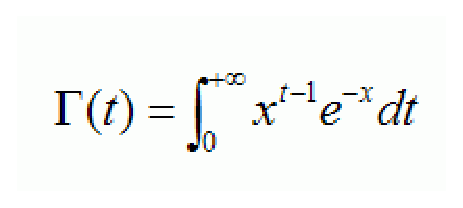
\includegraphics[scale=.5]{img/jsim/eulergamma.eps}
\end{center}

When r is a real non null positive integer, as in the  case of the Erlang distribution,
the Eulero function reduces  to $\Gamma$ (r)=(r-1)!
A random variable (r.v.) with Erlang distribution  of order \emph{r} can be obtained as a sum of \emph{r} exponentially  distributed random variables with mean 1/r$\alpha$.
\begin{center}
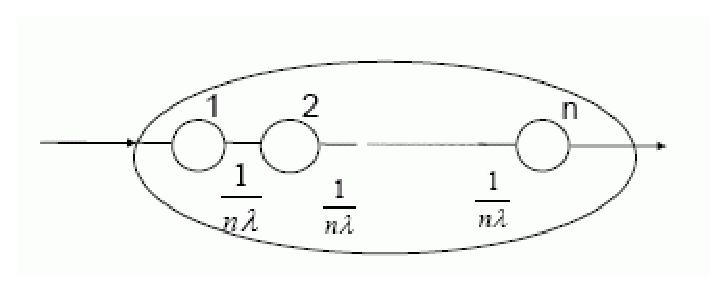
\includegraphics[scale=.5]{img/jsim/erlang2.eps}
\end{center}
When you change the values of $\alpha$ and r, the system  will automatically adjust the mean = r/$\alpha$ and the variance $\sigma ^ 2$ = r/$\alpha ^ 2$.
A family of probability density functions that illustrate the impact of various $\alpha$, r) pairs is shown below.\\
\begin{center}
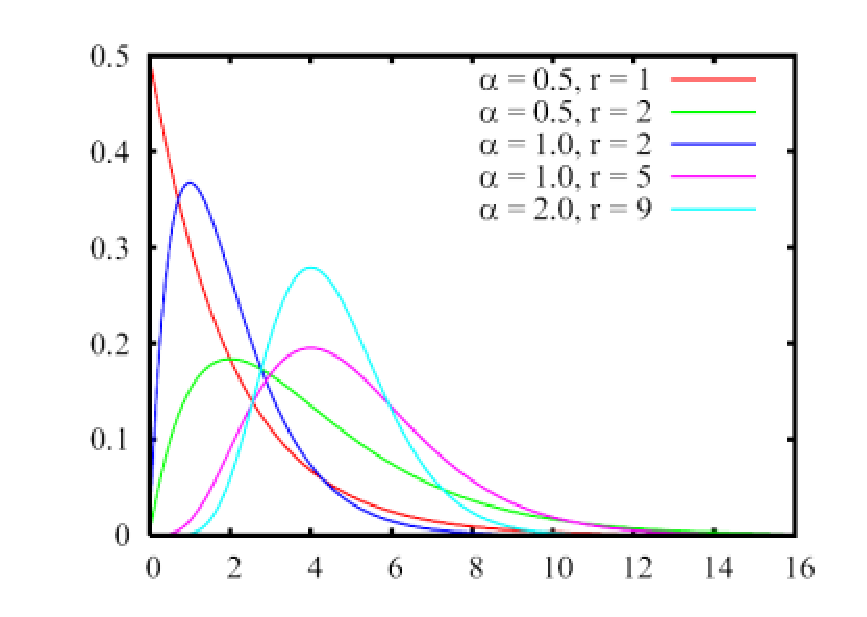
\includegraphics[scale=.5]{img/jsim/erl_pdf.eps}
\end{center}
% DISTR %
\textbf{Exponential}: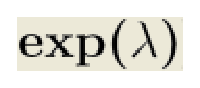
\includegraphics[scale=.5]{img/jsim/exponential_f.eps}\\\\
Probability density function\\
\begin{center}
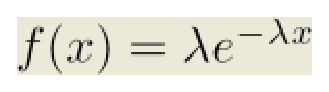
\includegraphics[scale=.5]{img/jsim/exponential1.eps}
\end{center}
This is a continuous probability distribution where $\lambda$ $>$ 0 is the distribution parameter, often called the \emph{rate} parameter; the distribution is supported on the interval [0,$\infty$).\\
The exponential distribution is used to model Poisson  processes, which are processes describing state changes of a system that occur  with constant probability per time unit $\lambda$.In this case, the time interval between two consecutive changes is
described by an exponential random variable with parameter $\lambda$.Therefore, if the system is in state A at time \emph{t = 0}, the integral of \emph{f(t)} from 0 to \emph{T} over \emph{t} represents the  probability that the system is in state B at
time \emph{t = T}. When you select this distribution, the parameter $\lambda$ is requires (real number) and the mean is computed as 
\includegraphics[scale=.3]{img/jsim/exponential2.eps} while the variance is 
\includegraphics[scale=.3]{img/jsim/expo_var.eps}.\\
A family of probability density functions is shown below, for a set of $\lambda$ values.\\
\begin{center}
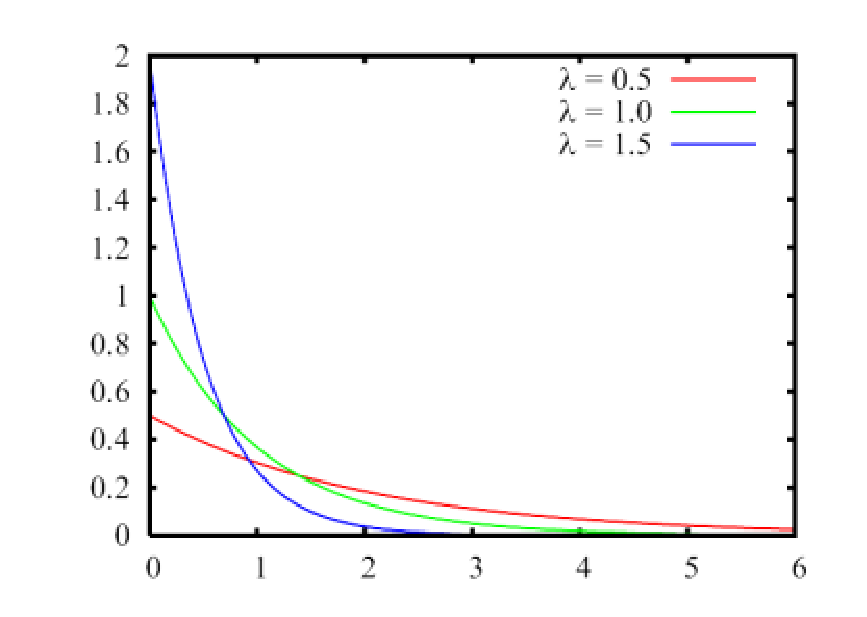
\includegraphics[scale=.5]{img/jsim/exp_pdf.eps}
\end{center}
\textbf{Gamma}: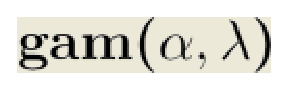
\includegraphics[scale=.5]{img/jsim/gamma_f.eps}\\\\
Probability density function\\
\begin{center}
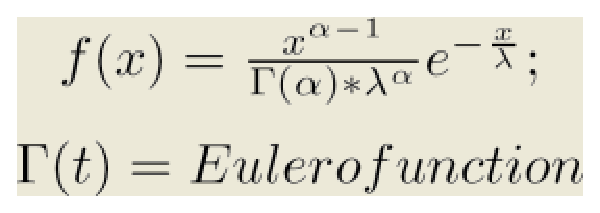
\includegraphics[scale=.5]{img/jsim/gamma1.eps}
\end{center}
This is a continuous probability  distribution. The parameters are the \emph{shape} $\alpha$ and the \emph{scale} $\lambda$, both real numbers.When you choose the Gamma distribution, you can either provide $\alpha$ and $\lambda$ or the distribution mean, equal to $\alpha$ * $\lambda$   and the variance $\alpha$ * $\lambda ^ 2$.
A family of probability density functions is shown below, for a set of $\alpha$ and $\lambda$ values.
\begin{center}
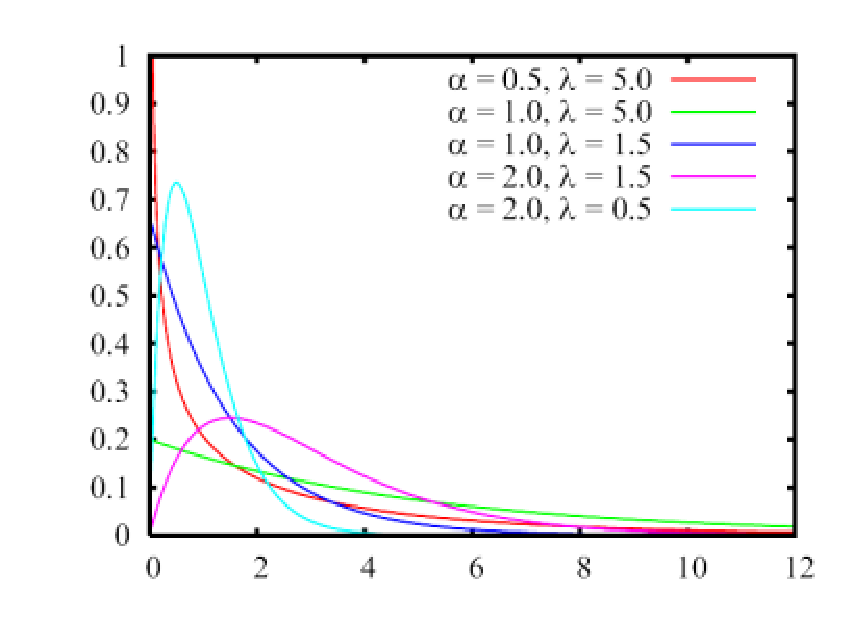
\includegraphics[scale=.5]{img/jsim/gamma_pdf.eps}
\end{center}
\textbf{Hyperexponential}: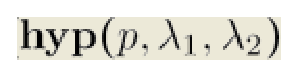
\includegraphics[scale=.5]{img/jsim/huperexpon_f.eps}\\\\
Probability density function\\
\begin{center}
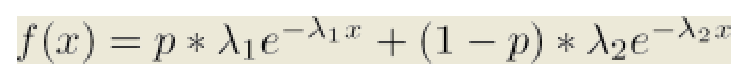
\includegraphics[scale=.5]{img/jsim/huperexpon1.eps}
\end{center}
A hyperexponential distribution describes a random  variable similar to an exponential but with more variability since it is the result of a weighted sum of two independent exponentially distributed  random variables, with paramters $\lambda$1 and $\lambda$2 respectively.The weight is the probability P that the random variable behaves like the exponential variable with parameter $\lambda$1 and 1-P that it behaves like the exponential variable with parameter $\lambda$2.\\
\begin{center}
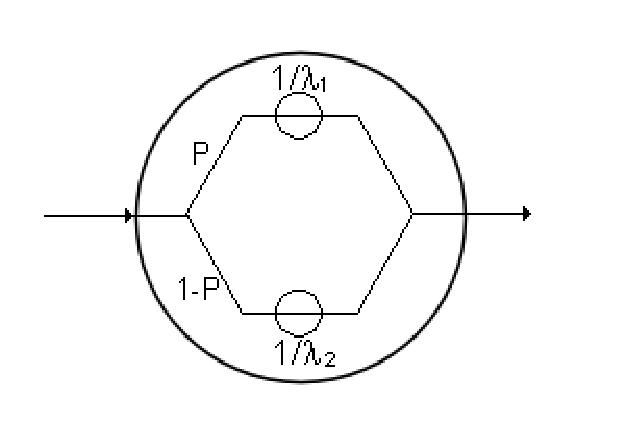
\includegraphics[scale=.5]{img/jsim/hyperExp1.eps}
\end{center}
When this distribution is used to model the customer interarrival time at a station (or the service time at that station), with  probability P the next interval before an arrival (service time) is  distributed like the upper branch in the figure above and with probability 1-P it will be distributed like the lower branch in the figure.
A family of probability density functions is illustrated in the picture below. Note that when $\lambda$1= $\lambda$2, the hyperexponential reduces to a simple exponential.\\
\begin{center}
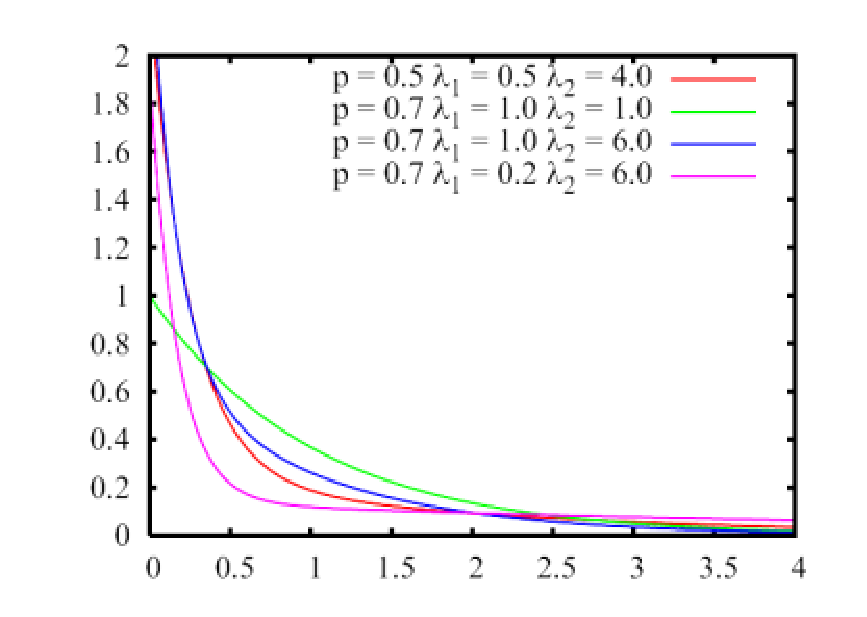
\includegraphics[scale=.5]{img/jsim/hyperexp_pdf.eps}
\end{center}
\textbf{Normal}: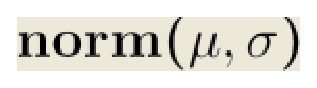
\includegraphics[scale=.5]{img/jsim/normal_f.eps}\\\\
Probability density function\\
\begin{center}
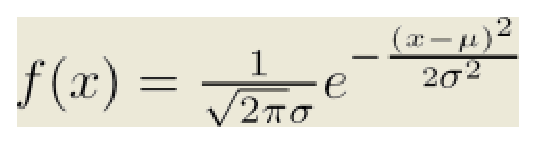
\includegraphics[scale=.5]{img/jsim/normal1.eps}
\end{center}
The Normal distribution is also called Gaussian since its probability density function is the Gaussian function.It is well known for its bell-shaped density function. The two parameters are $\mu$=location  (real number, it is the mean of the  distribution), and $\sigma$=scale (real number, it is the standard deviation of the distribution i.e. the square root of the variance).The density is symmetrical around the mean and the variance. The \textbf{standard} normal distribution is the normal distribution with $\mu$= 0 (mean equal 0) and $\sigma$ = 1 (variance equal 1).
A family of probability density functions is illustrated in the picture below. The standard distribution is depicted in green.\\
\begin{center}
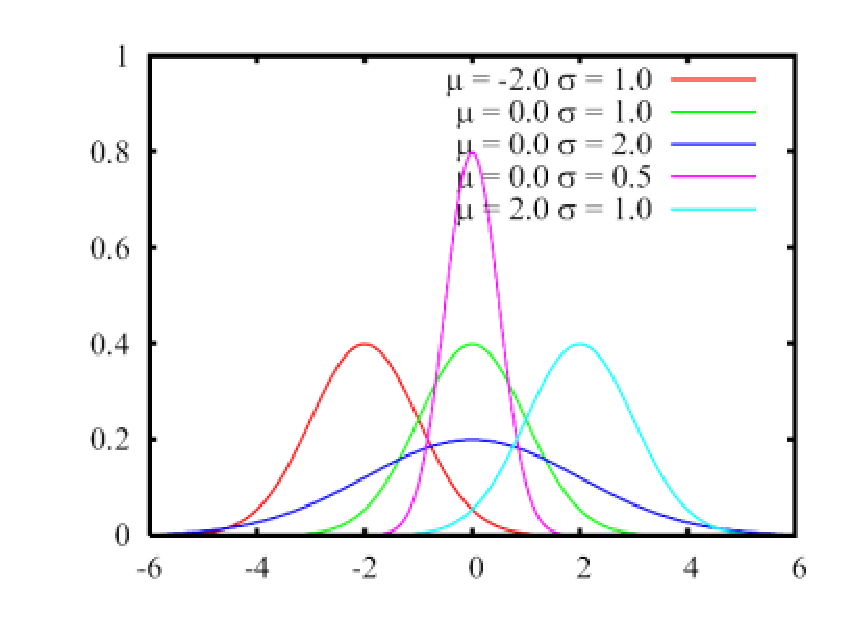
\includegraphics[scale=.5]{img/jsim/norm_pdf.eps}
\end{center}
\textbf{Pareto}: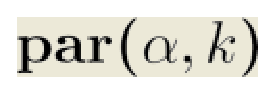
\includegraphics[scale=.5]{img/jsim/paretp_f.eps}\\\\
Probability density function\\
\begin{center}
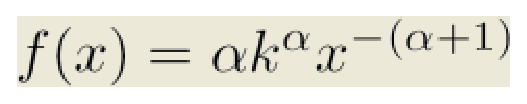
\includegraphics[scale=.5]{img/jsim/pareto1.eps}
\end{center}
This distribution usually describes  social and economical phenomena (typically, the distribution of wealth, where a small portion of the people owns the larger part of the wealth).It is charcaterized by the parameters k $>$ 0, location (real) and  $\alpha$ $>$ 0 shape (real).
When requested to input the distribution parameters, if k and $\alpha$ are provided, the system automatically derives the  mean m = \emph{k*$\alpha$ / ($\alpha$ - 1)} for k $>$ 1 and the variance c 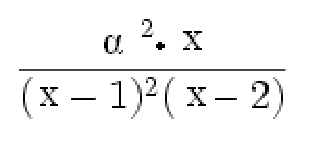
\includegraphics[scale=.5]{img/jsim/pareto_c.eps}.A famility of probability density functions  is illustrated in the picture below:\\
\begin{center}
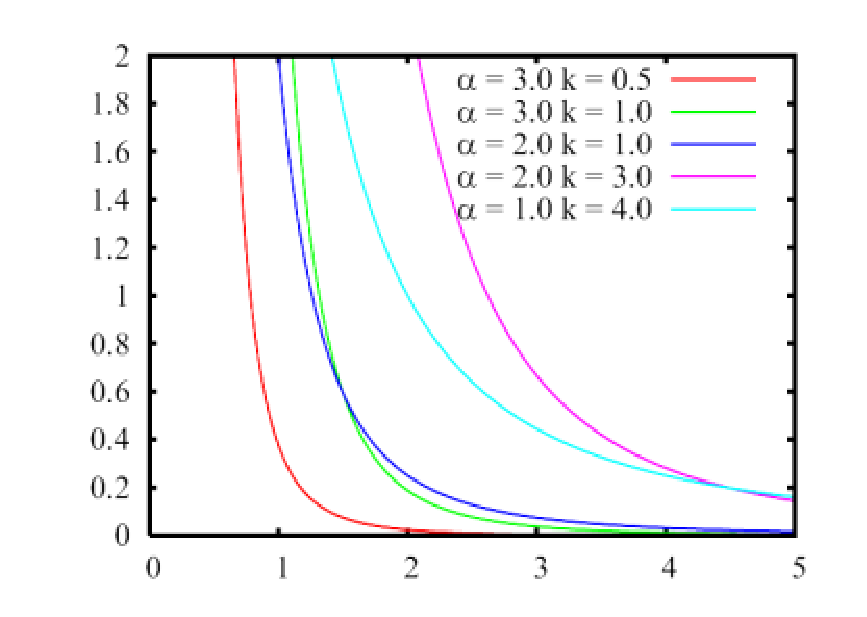
\includegraphics[scale=.5]{img/jsim/par_pdf.eps}
\end{center}
\textbf{Poisson}: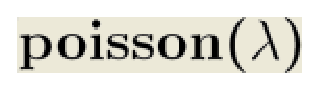
\includegraphics[scale=.5]{img/jsim/poisson_f.eps}\\\\
Probability density function\\
\begin{center}
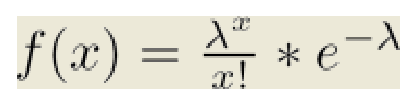
\includegraphics[scale=.5]{img/jsim/posson1.eps}
\end{center}
The Poisson distribution describes the number of events occurring over a given time interval, when such events are independent of  the amount of time elapsed and they occur at a fix average rate.It is a discrete probability distribution characterized by a single parameter, $\lambda$, a positive real number, which is the average number of  events in a time unit and its variance.
Thus, the probability of having an arrival in a time interval (t, t+$\Delta$t) is $\lambda$$\Delta$t + O($\Delta$t)), while the probability of more than one  arrival in the same interval is O($\Delta$t).For large time intervals, the distribution is near the mean value, thus the number n or arrivals over the interval is given by n = $\lambda$*T, where T is the length of the interval
A characteristic of the Poisson distribution is that the time intervals between two consecutive events is exponentially distributed with average $\Delta$.
The parameter $\lambda$ is not only the \emph{mean} number of occurrences but also its variance.
A family of probability density functions is illustrated in the picture below.\\
\begin{center}
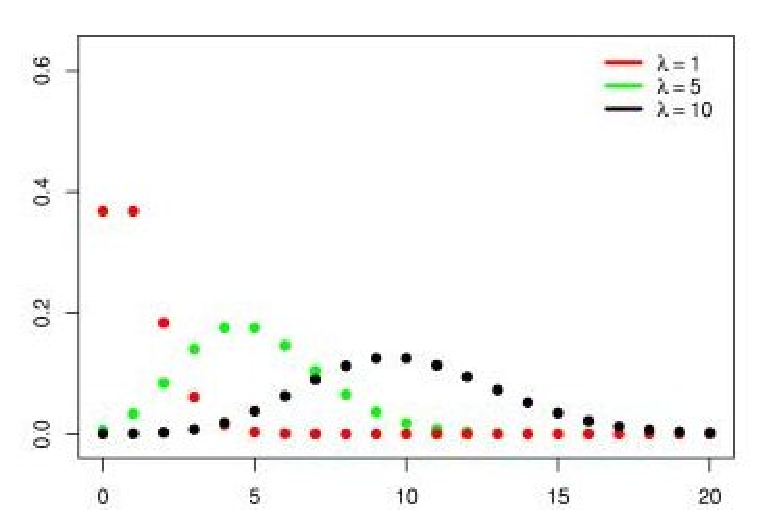
\includegraphics[scale=.5]{img/jsim/poisson_pdf_d.eps}
\end{center}
\textbf{Replayer}: 
\includegraphics[scale=.5]{img/jsim/replayer_f.eps}\\\\
When Replayer is chosen, a trace of data can be played back as the source of the distribution for service times or interarrival times.The file format is text/binary with values separated by CR (Carriage Return).In order to use this distribution, provide the absolute path name of the file in the input window.\\
\textbf{StudentT}:
\includegraphics[scale=.5]{img/jsim/studentT_f.eps}\\\\
Probability density function\\
\begin{center}
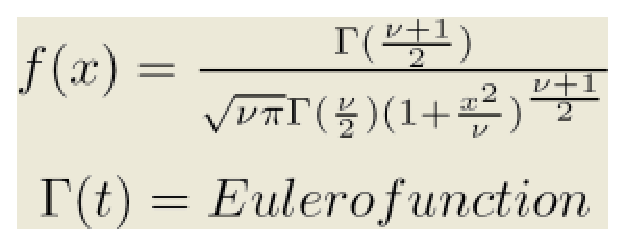
\includegraphics[scale=.5]{img/jsim/studentT1.eps}
\end{center}
The t-distribution, or Student t-distribution, is a continuous
distribution characterized by the single parameter $\upsilon$, a
real positive number. It is used when the mean of a normally
distributed population must be estimate using only a small sample
size. It is the basis of the Student-t's test that is used ot
evaluate the statistical significance of the difference between
two sample means and for the difference between two population
means.It is a special case of the generalized hyperbolic
distribution.The mean is 0 for $\upsilon$ $>$ 1 and the variance
is $\upsilon$/($\upsilon$ -2) for $\upsilon$ $>$ 2 (infinite
otherwise).
A family of probability density functions  for a set of $\upsilon$ values are illustrated in the picture below.\\
\begin{center}
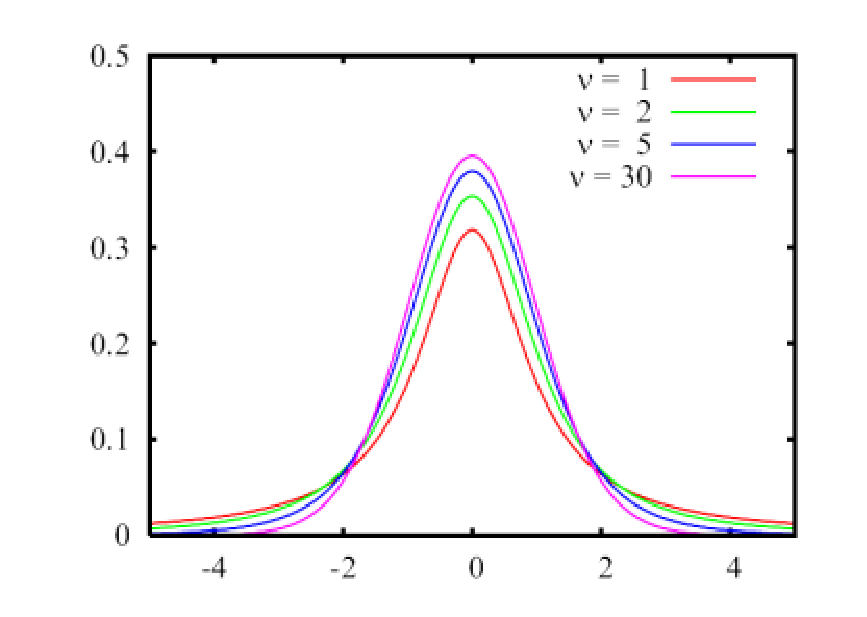
\includegraphics[scale=.5]{img/jsim/studentt_pdf.eps}
\end{center}
\textbf{Uniform}:\includegraphics[scale=.5]{img/jsim/uniform_f.eps}\\\\
Probability density function\\
\begin{center}
\includegraphics[scale=.5]{img/jsim/uniform1.eps}
\end{center}
The Uniform distribution is sometimes called rectangular due the shape of its density function.It describes a random variable that can assume values over the range
(\emph{min, max}), its characterizing parameters, with constant probability equal to 1/(\emph{max - min}).The probability is 0 outside the range.When you choose this distribution, you can either provide the pair (\emph{min, max}) or the mean m = (\emph{max + min})/2 and variance c = $(\emph{max - min})^2 / 12$.
The probability density function is plotted in the figure below.
\begin{center}
\includegraphics[scale=.5]{img/jsim/uniform_pdf.eps}
\end{center}

\subsection{Define stations}
\label{sec:DefineStations}
When you create a new model, you must define the Stations from the \textbf{Stations} page of the tabs menu.\\
\begin{center}
\includegraphics[scale=.5]{img/jsim/define_station1.eps}
\end{center}
You can insert one station at a time, by pressing the \includegraphics[scale=.5]{img/jsim/button_addStation.eps} button, or multiple stations all at once, by choosing the desired number in the input form \includegraphics[scale=.5]{img/jsim/button_Nstations.eps}
The added stations will be listed in the page. Various types of stations are available, the default type being \emph{server}.
If you want to remove any of the stations, select the target and press the corresponding \includegraphics[scale=.5]{img/jsim/delete.eps} delete button.
Stations are name Station1, Station2, and so on by default. If you want to assign model-relevant names, left-clik on a name to change and replace
it.
Similarly, if the default station type Server is not what you need, select from the drop down menu of each station the correct type.\\
\begin{center}
\includegraphics[scale=.5]{img/jsim/station_types.eps}
\end{center}
You can choose among the following types of station:
\begin{enumerate*}
\item \textbf{Delay station:} \includegraphics[scale=1]{img/jsim/delay.eps}\\
Customers that arrive at this station are delayed for the amount of time that defines the station service time. They do not experience any queueing, since a delay station is modelled as a station with an infinite number of servers with identical service time. Because customers never have to wait for service, response time at delay
stations is equal to service time, \emph{Ri = Si}. Furthermore, the queue length corresponds in this case to the number of jobs receiving service since there is no waiting:\\
\emph{Qi = RiXi = SiX = Ui. }
The utilization of the delay center represents the average number of jobs receiving service.
Delay centers are used when it is necessary to force some known average delay. A common application of delay centers is to model
transmission time of large amounts of data over a dedicated low speed transmission line.\\\\
In the Station Parameters tab menu page, you can modify:
\begin{description*}
\item[Service Section:]
in this section you can choose the service time distribution for the station.
For more information, see Service section \autoref{sec:ServiceSection}.
\item[Routing Section:]
in this section you can specify how serviced customers should be routed to the next station they will visit in the model.
For more information, see Routing section \autoref{sec:RoutingSection}.
\end{description*}
\item \textbf{Server station:} \includegraphics[scale=1]{img/jsim/server.eps}\\
The Server station is one of the most important components in a queuing network model. Service stations represent the service facilities of the system being modelled. A server station provides the required service to its customers. Server stations may have any (finite) number of servers. If all the servers in the service station are busy when a customer arrives at the station, the arriving customer is put in a waiting queue until its turn to receive service from the first available server is up.
The queueing discipline decides which customer is served next when a server becomes free. Therefore, the response time at server stations includes service time and
queuing time. Server stations may have more than one server. Their number is a parameter to be specified (default is 1).\\\\
In the Station Parameters tab menu page, you can modify:
\begin{description*}
\item[Queue Section:]
in this section you can choose the type of queue (finite or infinite) and the policy used to select the next customer to be served.
For more information, see Queue section \autoref{sec:QueueSection}.
\item[Service Section:]
in this section you can choose the service time distribution for the station.
For more information, see Service section \autoref{sec:ServiceSection}.
\item[Routing Section:]
in this section you can specify how serviced customers should be routed to the next station they will visit in the model.
For more information, see Routing section \autoref{sec:RoutingSection}.
\end{description*}
\item \textbf{Fork station:} \includegraphics[scale=1]{img/jsim/fork.eps}
A JSIM Fork station is simply a station where jobs are split into tasks. No service is provided, therefore there is no service time specification. Tasks are then routed along the Fork station outgoing links.
Unlike classical queueing theory fork-join queues, a JSIM Fork station is not associated with a join station automatically. Any combination of server stations, finite regions, fork-join, routing stations, etc., is possibile after a Fork station. This feature allows the modeling of very general parallel behaviors, of
which the traditional Fork-Join one is a special case. In JSIM the classical queueing theory Fork-Join queue behavior is obtained by connecting the Fork station to as many Server stations as the degree of parallelism requested, with one task per outgoing link. Each Server station is then connected to a Join station, where the job is
recomposed.
A Fork station is characterized by the forking degree, i.e., the number of tasks routed on each one of its outgoing links, and the capacity,
i.e., the maximum number of jobs that can be served by the station simultaneously. Therefore, the number of sibling tasks a job is split into is given by the product of the number of outgoing links from the Fork station times the forking degree. Note that a finite station capacity makes sense only when there is a join station downstream from the fork station that can recompose the split jobs. Otherwise, inconsistencies in the model and subsequent simulation error, such as out-of-memory, may occur. No automatic checks are available at the moment that can identify such critical conditions. Both the forking degree and the capacity are section parameters to be
specified in the model. As an example, a Fork station with forking degree 1, connected to three Server stations, would split a job into 3 sibling tasks (this is a traditional Fork-Join like behavior). If no Join station is connected to any of the three Servers, a warning message is displayed since the model could quickly saturate due to the extra load (3 more jobs) created in addition to each job entering the Fork station.\\\\
In the Station Parameters page of the tabs menu,you can modify:\\
\begin{description*}
\item[Fork Section:] in this section you can choose the forking degree of a job on each outgoing link and the fork station capacity, i.e., the maximum number
of jobs that can be served in parallel by the station.
For more information, see Fork section \autoref{sec:ForkSection}.
\item[Queue Section:] in this section you can choose the type of queue (finite or infinite) of the fork station in case its capacity is finite and jobs must wait before
proceeding through the fork station.
For more information, see Queue section \autoref{sec:QueueSection}.
\end{description*}
\item \textbf{Join station:} \includegraphics[scale=1]{img/jsim/join.eps}Join stations are complementary to fork stations.
In classical queueing network theory, a task arrives at a join station from the corresponding Fork station. In JSIM, a Join station may have incoming links from stations other than the corresponding Fork one. A Join station has no service time, as it is only used to recombine the tasks a job had been previously split into and then route the job to some other station(s). When a task arrives at a join station, it waits until all its sibling tasks have arrived. At this time, the original job is
recomposed and routed to the next station. If a job arrives from a station other than the corresponding Fork, i.e., a job that was not split, it is simply routed to the next station. In this case the Join station operates as a routing station.\\\\
In the Station Parameters tab menu page, you can modify:
\begin{description*}
\item[Routing Section:] in this section you can specify how serviced customers should be routed to the next station they will visit in the model.
For more information, see Routing section \autoref{sec:RoutingSection}.
\end{description*}
\item \textbf{Routing station:} \includegraphics[scale=1]{img/jsim/load_splitter.eps}
A routing station is a dummy station, with service time equal 0, that is used to create more complex and sophisticated routing strategies by sending jobs through one or more such stations. For example, if we wanted two thirds of the incoming traffic at station Z to be randomly routed to either station A or B and the remaining third to go either to station C or D, depending on the shortest queue at the two stations, we could implement the following. Add a routing station, Y, among Z's output stations and define random routing for the three of them (A, B, Y).
Then connect Y to C and D and define Join the Shortest Queue routing to C and D.\\\\
In the Station Parameters tab menu page, you can modify:
\begin{description*}
\item[Routing Section:] in this section you can specify how serviced customers should be routed to the next station they will visit in the model.
For more information, see Routing section \autoref{sec:RoutingSection}.
\end{description*}
\item \textbf{Source station:} \includegraphics[scale=1]{img/jsim/source.eps}
If the model comprises at least an open class, a sink and  a source stations are created by default, as they are necessary for the simulation and cannot be removed\\
\begin{center}
\includegraphics[scale=.5]{img/jsim/source_sink.eps}
\end{center}
Open classes are characterized by an infinite stream of jobs that can enter the system. Source stations are used to introduce jobs in the model. Their service time is the interarrival time of each customer class and as such, it is defined as a parameter of the class the job belongs to. The routing strategy defines the first station
a newly created job will visit. Only open class jobs can be routed from source stations.\\\\
In the Station Parameters tab menu page, you can modify:
\begin{description*}
\item[Routing Section:] in this section you can specify how newly created customers should be routed to the next station they will visit in the model.
For more information, see Routing section \autoref{sec:RoutingSection}.
\end{description*}
\item \textbf{Sink Station:} \includegraphics[scale=1]{img/jsim/sink.eps}\\
Open class customers leave the system once they have received all the service the need. Sink stations are used to model customers leaving the system, as they
enter the sink station but do not ever leave it. Sink stations have no parameters, only incoming connections from one or more stations, depending upon the model.
\end{enumerate*}

\subsubsection{Fork section}
\label{sec:ForkSection}
\textbf{How to define the Forking Behavior}
This section is characteristic only of fork stations. It defines the parallelism degree of a job, in terms of the number of tasks it is split into and how many jobs can be serviced simultaneoulsy.

In this section you can define the station forking degree, i.e., the number of tasks created for each job arriving at the fork station, and its capacity, i.e., the maximum number of of jobs that can be in a fork-join section (when a join is present):\\
\begin{center}
\includegraphics[scale=.5]{img/jsim/fork1.eps}
\end{center}
\emph{Forking degree:} it is the number of tasks that are routed on each outgoing link of the fork station. Therefore, each job is split into (forking degree)*(number of outgoing links) tasks. By default the forking degree is 1 and it can be modified using this form:\\
\begin{center}
\includegraphics[scale=.5]{img/jsim/tasks.eps}
\end{center}
\emph{Capacity:} it is the maximum number of jobs that can be served by a fork-join
section simultaneously. It makes sense only if there is a join station matching the fork one. It can be finite, in which case once the limit is reached, jobs wait in the queue of the fork station. A job is removed from the queue and serviced (i.e., split into tasks) when a job is recomposed at the matching join station and leaves it. Capacity is defined using the form below, after checking the \emph{Finite capacity...} box:\\
\begin{center}
\includegraphics[scale=.5]{img/jsim/blocking.eps}
\end{center}

\subsubsection{Queue section}
\label{sec:QueueSection}
\textbf{How to Define the Queue Strategy}\\
The Queue section is part of the \textbf{Station Parameters} definition page; it is present only for server and fork stations.

The Queue section allows the specification of the queueing capacity (whether finite or infinite) and policy. Different classes may have different policies associated with them.
\begin{center}
\includegraphics[scale=.5]{img/jsim/queue_section1.eps}
\end{center}
\emph{Capacity:} a station can accept any customer and let them
wait in queue, in which case its capacity is considered infinite,
or it can only accept a finite number
of customers. In this case its capacity is finite, with a length to be specified in the form \includegraphics[scale=.5]{img/jsim/lenght.eps}\\\\
\emph{Queue policy:}it is the algorithm used to decide which customer to serve next. A variety of factors can contribute to the order in which customers are served, such as arrival order, priorities associated with a class, the amount of service already provided to customers, etc.

In JSIM queueing disciplines based on arrival order and priority are the only available, namely:

\begin{description*}
\item[FCFS:] under the First Come First Served queueing discipline, customers are served in the order in which they arrive at the station. If the model is exported to MVA, the following constraint is enforced in the exported model. Since all customer classes must have the same average service time at a FCFS station, the total number of visits to the station (Vc,k) is adjusted in order to comply with the constraint and at the same time allow for distinct service demands (Dc,k).
\item[FCFS (Priority):] under this policy, customers are ordered according to their arrival time but customers with higher priority jump ahead of customers with lower priority (conventionally a \emph{small} priority number = low priority). Customers with the same priority are served FCFS.
\item[LCFS:] under the Last Come First Served queueing discipline, an arriving job jumps ahead of the queue and will be served first, unless other jobs arrive before the one currently in service finishes. The LCFS discipline implemented in JSIM is not the preemptive-resume type.
\item[LCFS (Priority):] under this policy, the next customer to be served is one with the highest priority (conventionally a \emph{small} priority number = low priority), so an arriving customer can only jump ahead of the queue of the other jobs with the equal or smaller priority. Customers with the same priority are served LCFS.
\end{description*}

\subsubsection{Routing section}
\label{sec:RoutingSection} \textbf{How to Define the Routing
Strategy} The Routing section is part of the \textbf{Station
Parameters} definition page defined for all stations, except for
fork and sink stations. In the routing section, for every class
defined, you may decide how the completed jobs are routed to the
other devices connected to station for which the routing strategy
is defined.
\begin{center}
\includegraphics[scale=.5]{img/jsim/routing1.eps}
\end{center}
For each class, the routing algorithm to be used on the outgoing links of the station is selected from this menu:\\
\begin{center}
\includegraphics[scale=.5]{img/jsim/strategy.eps}
\end{center}
By clicking an algorithm, a brief explanation of the selected algorithm is shown and routing options can be specified,where necessary:
\begin{center}
\includegraphics[scale=.5]{img/jsim/routing2.eps}
\end{center}
You can choose among the following algorithms (NOTE: in each of the pictures illustrating the algorithms, the blue station implements the routing strategy to the other devices):
\begin{description*}
\item[Random:] with this strategy, jobs are routed randomly to one of the stations connected to the routing device. The outgoing links are selected with the same probability.The figure illustrates the routing strategy with 3 output links. For each link the probability to be selected is 1/3.
\begin{center}
\includegraphics[scale=.5]{img/jsim/random.eps}
\end{center}
\item[Round Robin:] with this algorithm, jobs are cyclically routed to the outgoing links according to a circular routing. As the figure shows, the first job is sent to the top station, the second job is sent to the central station, and the third job is sent to the bottom station. The next job would be sent to the top station again, and so on.
\begin{center}
\includegraphics[scale=.5]{img/jsim/round_robin.eps}
\end{center}
\item[Probabilities:] with this algorithm, you can define the routing probability for each outgoing link.The sum of all probabilities must equal 1. If the values provided do not satisfy the constraint, JSIM automatically normalizes the values before the simulation starts.
\begin{center}
\includegraphics[scale=.5]{img/jsim/probability.eps}
\end{center}
This strategy requires that you define the probability for each
output link via the panel on the bottom right of the window.
\begin{center}
\includegraphics[scale=.5]{img/jsim/prob1.eps}
\end{center}
\item[Join the Shortest Queue:] with this strategy, each job is
routed to the device that has the smallest queue length, i.e.,
number of jobs waiting, at the time the job leaves the routing
station. The figure shows a case where the queue lengths at the
devices are 3, 2, and 1 jobs, respectively, from top to bottom.
The exiting job will be routed to the bottom station, since its
queue is the shortest(1 job).
\begin{center}
\includegraphics[scale=.5]{img/jsim/Q_length.eps}
\end{center}
\item[Shortest R Time:] with this algorithm, jobs are sent to the station where the average response time for the job's class is the smallest at the moment a job leaves the routing station.The figure shows that at the time of routing, the middle station has the smallest average response time, R, so the job will be sent to it.
\begin{center}
\includegraphics[scale=.5]{img/jsim/R_length.eps}
\end{center}
\item[Least Utilization:] with this strategy, the destination device is chosen as the one with the smallest average utilization at the time routing is performed. In the example depicted in the picture, the top station is the least utilized, so it will receive the next job to leave the blue station.
\begin{center}
\includegraphics[scale=.5]{img/jsim/utilization.eps}
\end{center}
\item[Fastest Service:] with this strategy, a job is routed to the device with the smallest average service time, S, for the job's class. In the figure, the exiting job will be routed to the top station since it service time is the minimum among the three.
\begin{center}
\includegraphics[scale=.5]{img/jsim/S_time.eps}
\end{center}
\end{description*}

\subsubsection{Service section}
\label{sec:ServiceSection}
\textbf{How to Define the Service Strategy}
This section is present in server and delay stations.
This section allows the specification of the number of servers, for server stations, and the service time distribution, for both server and delay stations.

Delay stations are infinite servers with identical service time, therefore they only need the service time distribution. The infinite number of servers provides for equal average response time for all jobs, as no job waits in queue for service.

In this section, the load dependent or independent nature of the service time is also specified for each class in server stations:
\begin{center}
\includegraphics[scale=.5]{img/jsim/service_section1.eps}
\end{center}
The number of servers in a server station can be modified using the corresponding input area:
\begin{center}
\includegraphics[scale=.5]{img/jsim/num_servers.eps}
\end{center}
For each class, you must specify whether the service time is Load Dependent or Load Independent using this menu:
\begin{center}
\includegraphics[scale=.5]{img/jsim/load.eps}
\end{center}
A load independent service indicates that, regardless of the number of jobs that are in the station, the system will serve all jobs following a fixed policy modelled by the chosen statistical distribution.\\
For each class, the Service Time Distribution is set to Exponential with average equal to 1. It can be modified by clicking the  \includegraphics[scale=.5]{img/jsim/edit.eps} button and inserting all the required parameters from this window:
\begin{center}
\includegraphics[scale=.5]{img/jsim/erlang.eps}
\end{center}
Click the drop down menu and choose the service time distribution among the following:
\begin{itemize*}

\item Burst (general) \item Constant \item Erlang \item
Exponential \item Gamma \item Hyperexponential \item Normal \item
Pareto \item Poisson \item Replayer \item StudentT \item Uniform
\end{itemize*}
A load dependent service time indicates that the amount of time the server spends with each customer depends upon the current number of customers in the station. A set of intervals for the number fo jobs in the station is specified, either by adding one range at a time via the \includegraphics[scale=.5]{img/jsim/add_range.eps} button or by specifying the total number at once. Each range must them be specified by its lower (From) and upper (To) extremes. Each such range can be associated with different service times, as for the distribution, the mean and the coefficient of variation, or a subset thereof.
To set the parameters of a Load Dependent service time, click the \includegraphics[scale=.5]{img/jsim/edit.eps} button and then specify the parameters for each added range.
\begin{center}
\includegraphics[scale=.5]{img/jsim/load_dipendent.eps}
\end{center}
For each customer number range you must specify the following parameters:
\begin{description*}
\item [Distribution:] you can choose among Burst (general),
Pareto, Erlang, Exponential, Hyperexponential, Poisson, Uniform,
Constant, Gamma and Normal distribution. \item [Mean:] the mean
value of each distribution is specified in the \emph{Mean} form by
double clicking on it. Insert a number or an arithmetic expression
that will be evaluated with JFEP - Java Fast Expression Parser by
Bertoli Marco. For a complete list of the command supported by
JFEP you can read the \emph{Help} tab or see the official JFEP web
site at http://jfep.sourceforge.net/ \item [C:] The coefficient of
variation of each distribution (when C exist) can be specified by
double clicking on the \emph{C} form. For example, in the previous
picture two policies are defined: From 1 to 4 jobs in the station,
the server will behave according to an Erlang distribution with
mean = 1 and C = 0.5. For any number of jobs greater or equal to 5
in the station, the system will behave according to an Exponential
distribution with mean = 1. If you want to delete a range click
\includegraphics[scale=.5]{img/jsim/delete.eps}
\end{description*}

\subsection{Define Connections}
\label{sec:DefineConnections}
The \textbf{Connections} tab allows you to define how stations are connected with each other.
In order to create a connection from station \emph{i} to a station \emph{j}, check the table entry (i,j) in the connection matrix (rows identifiy source stations, columns identify destination stations)
\begin{center}
\includegraphics[scale=.5]{img/jsim/connections1.eps}
\end{center}
\textbf{NOTE:} if there are open classes in the model, the Source and Sink station automatically created by the system appear in the connection matrix.  A Source station may have only outgoing links, a Sink station may have only incoming links.
\begin{center}
\includegraphics[scale=.5]{img/jsim/sink_source_connections.eps}
\end{center}
To define a consistent model a Source station must have at least one outgoing connection and a Sink station must have an incoming connection.\\\\
\textbf{Example 1:} if you want to connect station1 to station2 in this way \includegraphics[scale=.5]{img/jsim/es1.eps} you must check this box
\begin{center}
\includegraphics[scale=.5]{img/jsim/connection1.eps}
\end{center}
\textbf{Example2:} if you want to connect station1 to station2 in this way \includegraphics[scale=.5]{img/jsim/es2.eps} you must check this box
\begin{center}
\includegraphics[scale=.5]{img/jsim/connection2.eps}
\end{center}
\textbf{Example3:} if you want to connect station1 to itself (with a feedback loop) \includegraphics[scale=.5]{img/jsim/es3.eps} you must check this box
\begin{center}
\includegraphics[scale=.5]{img/jsim/connection3.eps}
\end{center}
\textbf{NOTE: }if connections among the stations are inconsistent, the system displays error-warning messages. For more information about connection errors, read ref{}.

\subsection{Station Parameters}
\label{sec:StationParameters}
The \textbf{Station Parameters} tab allows you to define the characteristic parameters of each station.
For each station, a different menu is presented depending upon the station type. Queuing, service, routing and forking, or subsets thereof, are the characteristics to be defined through a series of tabs. Default settings are provided that can be modified at the user's need. The Sink station does not have any parameter.
\begin{center}
\includegraphics[scale=.5]{img/jsim/station_parameters1.eps}
\end{center}
\textbf{Example }(with a server station):
\begin{center}
\includegraphics[scale=.5]{img/jsim/sub_tabs_menu.eps}
\end{center}
\textbf{NOTE:} You can find detailed information about station parameters \autoref{sec:DefineStations}.

\subsection{Define Performance Indices}
\label{sec:DefinePerformanceIndices}
Performance Indices are selected using the \textbf{Performance Indices} tab.
\begin{center}
\includegraphics[scale=.5]{img/jsim/define_indices1.eps}
\end{center}
You can choose any subset of indices from the list below to be
plotted as the model output:
\begin{description*}
\item [Queue Length] Number of customers at a station, both
waiting and receiving service. \item [Queue Time] Average time
spent by the customers waiting in a station queue. It does not
include the Service Time. \item [Residence Time] Total time spent
at a station by a customer, both queueing and receiving service,
considering all the visits at the station. \item [Response Time]
Average time spent in a station by a customer for a single request
(it is the sum of Queueing time and Service time). \item [System
Response Time] Average time a customer spends in the system in
order to receive service from the various stations it visits. It
corresponds to the intuitive notion of response time, as the
interval between the submission of a request and the reception of
the response. \item [Utilization] Percentage of time a resource is
used w.r.t. the system lifetime; it varies from 0 (0\%), when the
station is always idle, to a maximum of 1 (100\%), when the
station is constantly busy serving customers for the entire system
lifetime. Utilization may be greater than 1 if a station has more
than one server. \item [Throughput] Rate at which customers
departs from a station, i.e., the number of services completed in
a time unit. \item [System Throughput] Rate at which customers
departs from the system. \item [Customer Number] Average number of
customers in the system. If the index is associated with a closed
class, then it is  equal to the number of customers in the class.
\end{description*}
Each index is associated with a class and a station and will be computed within a given Confidence Interval and Max Relative Error, both defined on the (0-1) range, by performing the following steps:
\begin{enumerate*}
\item Select the index you want to add to the model from this menu:
\begin{center}
\includegraphics[scale=.5]{img/jsim/indices1.eps}
\end{center}
\item Click \includegraphics[scale=.5]{img/jsim/add_indice.eps} and the index will be added to the panel. Next the index parameters must be set.
\item Select from the Class menu a single class, or All Classes, for which the index must be computed.
\begin{center}
\includegraphics[scale=.5]{img/jsim/classes.eps}
\end{center}
\item Select the Station for which the index must be computed from Station menu. In case of system wide indices, namely, System Throughput and System Response Time, this option is not available.
\begin{center}
\includegraphics[scale=.5]{img/jsim/station.eps}
\end{center}
\item Double click on the values to modify the default values for the Confidence Interval size of the solution and for the Max Relative Error of the greatest sample error, if you want more/less accurate results.
\begin{center}
\includegraphics[scale=.5]{img/jsim/err_conf.eps}
\end{center}
\item Repeat these steps for all the indices you want to include in the model output.
\end{enumerate*}
\textbf{NOTE:} erroneous parameter settings will be detected only when the simulation is started, raising a warning or an error message.

\subsection{Reference Stations}
\label{sec:ReferenceStations}
The \textbf{Reference Stations} tab allows you to specify the Reference Station for each customer class.
For each customer class, a reference station must be specified in order to compute system throughput for that class. For open classes, there is only one possible reference station, that is, the Source station. Such an association is done by the system automatically each time an open class is created and cannot be modified.
\begin{center}
\includegraphics[scale=.5]{img/jsim/open_reference.eps}
\end{center}
For each closed class, any of the existing stations can be selected using the scroll menu below
\begin{center}
\includegraphics[scale=.5]{img/jsim/closed_reference.eps}
\end{center}
\textbf{NOTE:} if a reference station is missing for any of the classes, an error message is returned when the simulation will start.

\subsection{Finite Capacity Regions}
\label{sec:FiniteCapacityRegions}
The \textbf{Finite Capacity Regions} tab allows you to define Finite Capacity Regions in the model.
Finite Capacity Regions can either be added one at a time by clicking the \emph{Add Region} button or all at once by selecting the desired number in the \emph{Regions} selector.
\begin{center}
\includegraphics[scale=.5]{img/jsim/add_fcr.eps}
\end{center}
When a new region is created, two new sub areas devoted to the parameters of the region, namely the stations involved and class properties when in the region, appear on the screen on the right.
\begin{center}
\includegraphics[scale=.5]{img/jsim/fcr_bottom.eps}
\end{center}
For each region, define first the capacity (infinite by default). If the check in the Infinity box is removed, the desidered number can be input in the Capacity field.
\begin{center}
\includegraphics[scale=.5]{img/jsim/fcr_selection.eps}
\end{center}
Then for each region define which stations are part of that region. Stations are added in alphabetical order on their names. If the model has more than one station, a drop down menu from the station name allows you to change the station to add.
\begin{center}
\includegraphics[scale=.5]{img/jsim/station_selection.eps}
\end{center}
Finally, in the bottom right panel, you can define class specific properties for the finite capacity region selected. Region capacity for that class (finite or infinite -the default value) and the dropping characteristic (true or false) in case the capacity is exceeded are defined here.
\begin{center}
\includegraphics[scale=.5]{img/jsim/class_selection.eps}
\end{center}

\subsection{Define Simulation Parameters}
\label{sec:DefineSimulationParameters}
The Simulation Parameters and Initial State of the model are defined using the \textbf{Simulation} tab.
\begin{center}
\includegraphics[scale=.5]{img/jsim/sim_tabs.eps}
\end{center}
\begin{description*}
\item [Simulation parameters:] In the top section of this windows
you can edit general simulation parameters.
\begin{figure}
\begin{center}
%\includegraphics[scale=.5]{img/jsim/first_section.eps}
\end{center}
\end{figure}

\item [Simulation Seed:] The simulation seed is a
number used by the simulation engine to generate pseudo-random
numbers. As this numbers are pseudo-random, if you change the
seed, you will obtain a different sequence of pseudo-random
numbers. If a simulation is repeated using the same seed, the same
sequence of pseudo-random numbers will be generated, thus leading
to identical results. The default value is random, which indicates
that the simulation engine will pick a seed of its choice in a
pseudo-random fashion each time it is started; deselect
\emph{random} and insert a number if you want a custom simulation.
\item[Maximum duration (sec):] It represents the maximum amount of
time in seconds that the simulation will run. If the simulation
ends before the maximum duration, the parameter is ignored and
does not affect the results. The default value is \emph{infinite}
deselect it and specify the preferred maximum time if you do not
want the simulation to run for a possibly very long time. In this
case, the simulation stops when the time limit is reached,
although a solution may not be available yet. \item [Maximum
number of samples:] It is the greatest number of samples for each
index that JSIM collects before ending the simulation. During a
simulation, measurements can be stopped in case of:
\begin{itemize*}
\item Success, if the results have reached the required Confidence Interval and the Max Relative Error
\item Failure, if the simulation has analyzed the maximum number of samples but has not reached the required Confidence Interval or Max Relative Error
\item Failure, if timeout occurs before successfully calculating the final results.
\end{itemize*}
The default value for the maximum number of samples is 500,000; you may increase it (for a more accurate simulation) o decrease it (for a faster simulation).
\item [Representation Interval (sec):] This is the granularity at which results are plotted on the screen, i.e., the time interval before a new point is added to the graphs, as the simulation proceeds. A large value will make the simulation to proceed slower, as the graphs are updated less often. Small values will provide an impression of better \emph{responsiveness} from the simulation, as graphs are updated more frequently.
\end{description*}
\textbf{Initial state:}
Initial state is the model situation at time 0, typically expressed by the number of customers in each station before starting the simulation. For closed customer classes, all jobs are initially allocated to their reference station. You can modify this allocation, as long as  the total number of jobs remains the one defined in the
Classes (\autoref{sec:DefineClasses}) tab.
For open customer classes, it is possible to initialize each station with any desired number of jobs. The following table represents an example of an initial state of a model with three stations and two classes.
\begin{center}
\includegraphics[scale=.5]{img/jsim/bottom_section.eps}
\end{center}

\subsection{Define what if analysis}
\label{sec:DefineWhatIfAnalysis}
The parameters of a what-if analysis are defined using the \textbf{What-if-analysis} tab.
\begin{center}
\includegraphics[scale=.5]{img/jsim/whatif_tab.eps}
\end{center}
A What-If Analysis consists of a series of simulations in which one or more parameters are varied over a specified range. This allows the observation of system behavior under a spectrum of conditions, unlike the single JSIM simulation run where the system is observed under a specific set of configuration parameters.
By default the what-if-analysis is not enabled. It must be activated explicitly and its parameters defined.
\textbf{Activating the What-If Analysis }\\
After completing the definition of the model and selecting the \textbf{What-if analysis} tab, check the Enable what-if analysis checkbox to activate it.
\begin{center}
\includegraphics[scale=.5]{img/jsim/enable_box.eps}
\end{center}
\textbf{Selecting the What-If Analysis Parameter}\\
After enabling the what-if analysis, it is possible to select the parameter to control the series of simulation runs using the menu below:
\begin{center}
\includegraphics[scale=.5]{img/jsim/type_selection.eps}
\end{center}
When you select a what-if analysis parameter, the bottom section
of the window will change depending upon the parameter. In the
right portion a description is provided of the selected parameter
and of the impact of its variation. In the left portion the
details of the parameter range (From and To fields) and the number
of executions (Steps) on the range are provided. The set of
modifiable parameters depends upon the number and type of classes
in the model:
\begin{itemize*}
\item In a single class model, you simply select the parameters you want to change during simulation.
\item In a multiclass model, you select the parameter and specify whether you want to apply the variation to all classes or just to one class.
\end{itemize*}

\textit{Number of Customers (only for models with closed classes)}
JSIM repeats the simulation changing the number of jobs in each run,
starting from the number inserted in the \emph{From N} field, to the value inserted
in the \emph{To N} field. The simulation is repeated \emph{Steps (n. of exec.)} number of times.
\begin{center}
\includegraphics[scale=.5]{img/jsim/customers.eps}
\end{center}
In the figure above a what-if analysis is planned on a single class model.
The initial value of the number of customers is not modifiable from this window, as it is part of the \textbf{Classes} tab. The final value is specified in the field \emph{To N}. In this case, with a final value
of 20 and 6 Steps, simulations are run for 10, 12, 14, 16, 18 and 20 customers, respectively. Only the customer number in the class selected in the \emph{Class} (Chiusa, in the picture) will be changed. The remaining classes will keep their initial number of customers. The simulator makes sure that the sum of the percentages of customers in various classes add up to 1, as shown in the \emph{Population mix} table on the bottom of the window.
If the \emph{all-classes} option is selected, the overall population is increased while keeping the relative proportion of jobs in the various classes constant. Because the number of customers in each class can only be an integer number, only the population vectors with integer components can be considered. Therefore, the actual number of executions may be smaller than the one specified.\\\\
\textit{Population Mix: (only for models with two closed classes)}
The population mix describes the way the population is divided
between the two class, i.e., the percentage of customers in each
class over the total population. Because of the complexity of the
underlying modelling, this type of analysis is possible only for
models with two closed classes. Mixed class models can be analyzed
too, as long as there are two closed classes. Only the closed
classes will be considered.
\begin{center}
\includegraphics[scale=.5]{img/jsim/popmix.eps}
\end{center}
In order to allow for a complete analysis of the population mix, in this case the initial value of the percentage of customers in one of the two classes, the one selected through the \textbf{Class} field, can be modified. Its default value is the ratio of the class population to the total population of closed customers, defined in the \textbf{Class} tab. Both the final and the initial \emph{beta} are numbers on the range [0-1].\\\\
\textit{Arrival Rate: (only if there are open classes)}
Arrival rate is the frequency at which jobs arrive at a station during a period of time.
Similarly to the number of customers, the arrival rate can be changed for one specific open class or for all the open classes in the model. If a single class is selected, the final arrival rate and the number of steps must be specified. The initial arrival rate is specified in the Arrival Rate section of the \textit{Classes} tab and it is not modifiable here.
If the arrival rate is to be changed for all classes, the final value is expressed as a percentage, which is applied to all classes.
\begin{center}
\includegraphics[scale=.5]{img/jsim/ex1.eps}
\end{center}
The figure above shows the settings for a what-if analysis on the arrival rate of all the open classes. The \emph{To} field is seto to 150\%, which means that for each class the final arrival rate will be one and a half times the initial value. 10 runs will be exectued with equally spaced (in percentage) intermediate values.\\\\
\textit{Service time (for all types of classes)}
Service Time is the time required by a customer class at each visit at a station. In this case, besides the final value and the number of runs to be executed, the station and the customer class (or all the classes) whose service time will be varied must be specified.
\begin{center}
\includegraphics[scale=.5]{img/jsim/ex2_service_time.eps}
\end{center}
The figure above shows the settings for a what-if analysis of the service time of class Class1 at station Server1. The service time distribution will not change. Only its average will be modified to span the range defined by the intial value (specified in the \textbf{Station Parameters} tab) and the final value specified here in
the \emph{To} field.
If the \emph{All classes} option is selected, the range of service time to explore is expressed in percetange, starting from the initial value specified at model definition (100\%). The station where the service time change is applied must be specified.\\\\
\textit{Seed (for all types of classes)}
\begin{center}
\includegraphics[scale=.5]{img/jsim/sedd.eps}
\end{center}
Unlike the previous cases, where the analysis is performed for a range of values of one of the model parameters in order to investigate the system behavior under a variety of conditions, a what-if analysis on the seed aims at evaluating the sensitivity of the simulation engine to numerical conditions, in particular to the initial value fed to the pseudo-random number generator, i.e., the seed.
The Simulation engine uses a pseudo-random number generator to generate the sequence of values used in each execution. By changing the seed, a different sequence of values is produced, thus leading to different numerical results. The first value is the one defined in the \textbf{Simulation Parameters} tab. In this panel, the number of executions is specified and the simulation engine generates as many pseudo-random seeds to be used in the executions.

\section{Import in JMVA}
\label{sec:importInJMVA}
After creating a simulation model, you can export it to the analytic solver component of the JMT suite, namely JMVA. In the Action menu, click \emph{Export to MVA}.
\begin{center}
\includegraphics[scale=.5]{img/jsim/import_to_JMVA.eps}
\end{center}
If there are errors in the model, i.e., conditions not allowed in models with analytical solution, a dialog window with information about such errors appears (See \autoref{sec:ErrorAndWarningMessages}). If you want to continue with the analytical solution, you must corret the errors.
When the model satisfies all the constraints for analytical solution, a JMVA window appears on the screen and the model can be solved with JMVA.
\begin{center}
\includegraphics[scale=.5]{img/jsim/jmva.eps}
\end{center}
Refer to JMVA user's guide (\autoref{cha:jmva}) for specific help on JMVA functionalities.

\section{Modify default parameters}
\label{sec:ModifyDefaultParameters} The simulator default settings
as for Class, Station, Simulation, and Finite Capacity Region
parameters, may be changed using the Define menu in the menu bar.
Click the \emph{Default parameters}
\begin{center}
\includegraphics[scale=.5]{img/jsim/define1.eps}
\end{center}
or the \includegraphics[scale=.5]{img/jsim/define2.eps}
\emph{Define default values of model parameters} button. In JSIM
all parameters have predefined, or default, values. Such values
can be change to suit the user's most common modelling activities.
Defaults can be modified for the following sections:
\begin{itemize*}
\item Class Parameters
\item Station Parameters
\item Simulation Parameters
\item Finite Capacity Region (FCR) Parameters
\end{itemize*}
\textbf{Class Parameters}
These settings define the default class parameters used when a new class is created. For detailed information about classes, see \autoref{sec:DefineClasses}.
\begin{center}
\includegraphics[scale=.5]{img/jsim/Class_Parameters.eps}
\end{center}
\emph{Name:} the default name for each newly created class of customers is \emph{Class}, followed by a progressive integer, starting from 1, indicating how many classes you have created so far. It can be reset to any alphanumerical string, which will be followed by the same numbering scheme.\\\\
\emph{Type:}
the default class type is Closed. If open classes are used more often, you may want to change to Open as default, so as to minimize the type changes in the class definition section.\\\\
\emph{Priority:}
the default class priority is 0. Higher numbers correspond to higher priority.\\\\
\emph{Population:}
this parameter applies only to \emph{closed classes}; the default value is 1, i.e., all closed classes are created with 1 customer in each of them. Change the value if you want larger populations by default in each closed class.\\\\
\emph{Distribution:}
this parameter applies only to <em>open classes; the default value is \emph{Exponential} since it is the most popular distribution that characterizes customer interarrival times at a system. Change it to any of the distributions available if most of your customer interarrival times follow a non-exponential pattern.\\\\
\textbf{Station Parameters}
These settings are general parameters for every type of station. For a detailed description of station types, see \autoref{sec:DefineStations}
\begin{center}
\includegraphics[scale=.5]{img/jsim/Station_parameters.eps}
\end{center}
\emph{Name:}
the default name of each newly created station is \emph{Station}, followed by a progressive integer, starting from 1, indicating how many classes you have created so far. It can be reset to any alphanumerical string, which will be followed by the same numbering scheme.\\\\
\emph{Type:}
the default station type is \emph{Server}, since this is the most popular type of station in performance models. Alternative types are \emph{Server}, Fork, Join, Routing, Delay.\\\\
\emph{Queue Capacity:}
this parameter applies only to \emph{Server} and \emph{Fork} station types; the default value is infinite, i.e., an infinite number can queue at such stations. It can be reset to finite, with a finite value specified, by checking out the Infinite checkbox.\\\\
\emph{Number of Servers:}
this parameter applies only to <em>Server stations; the default value is 1, as most devices are single server. It can be changed to any finite value.\\\\
\emph{Queue Strategy:}
this parameter applies only to <em>Server and <em>Fork station types; the default value is FCFS and can be changed to LCFS. In both cases, a priority version of the discipline is also available.\\\\
\emph{Service Distribution:}
this parameter applies only to <em>Server stations; the default value is Exponential, as it is the most popular when modelling device service time. It can be changed to any of the available distributions if most of the devices modelled are non-exponential.\\\\
\emph{Delay Service Distribution:}
this parameter applies only to \emph{Delay stations}; the default value is Exponential but i can be changed to any of the distributions available.\\\\
\emph{Routing Strategy:} this parameter applies only to <em>Delay,
Server, Join, and \emph{Routing stations}; the default value is
Random and it can be changed to any of the available routing
strategies, namely
Random, Round robin, Probabilities, Join the Shortest Queue, Shortest R time, Least utilization, and Fastest service.\\\\
\emph{Drop Rule:}
this parameter applies only to \emph{Fork stations}. When a finite capacity is defined, the default value of the Drop Rule is Drop, i.e., all customers exceeding the station capacity are discarded. Two other policies are possible. When the capacity is infinite, the Drop Rule is disabled by default.\\\\
\emph{Fork Capacity: }
this parameter applies only to \emph{Fork stations}; the default value is infinite, i.e., no limit on the number of customers entering a Fork station exists. It can be changed to finite, by checking the blocking checkbox and a finite number must then be specified.\\\\
\emph{Forking Degree: }
this parameter applies only to \emph{Fork stations}; the default value is 1, i.e., one task is generated for each outgoing link of the Fork station. It can be changed to any finite value, thus increasing the degree of parallelism a job has (and the number of tasks it is split into).\\\\
\textbf{Simulation Parameters}
These parameters define the simulation behavior from a statistical point of view. For more information, see \autoref{sec:DefineSimulationParameters} for simulation parameters or \autoref{sec:DefineSimulationParameters} for Confidence Interval and Max Relative Error.\\\\
\begin{center}
\includegraphics[scale=.5]{img/jsim/Simulation_parameters.eps}
\end{center}
\emph{Confidence Interval Measure: }
this parameter is set by default at 90\%, a commonly used value as it provides a good trade-off between results accuracy and simulation time; larger values will lead to more accurate results at the expenses of an increase in the time the simulation takes to complete, smaller values will achieve the opposite effect.\\\\
\emph{Max Relative Error Measure:}
this parameter is set by default at 10\%; smaller values will increase results accuracy while bigger values allow for larger errors in the samples.\\\\
\emph{Simulation Seed:}
this parameter is used to initialize the pseudo-random number generator; it should be changed very cautiously, since the statistical quality of the sequence of pseudo-randomly generated numbers is affected by the seed choice.\\\\
\emph{Maximum Duration:}
this parameter is set to infinite by default, so that even lengthy simulations can complete and satisfy even narrow confidence intervals; finite values (in seconds) may force termination before the end of the simulation.\\\\
\emph{Maximum Number of Samples: }
this parameter is set by default to 500,000; with a smaller number of samples it may not be possible to achieve the requested confidence interval, a larger number may not necessarily increase the results accuracy and simply extend the simulation time.\\\\
\emph{Animation Update Interval:}
this parameter indicates the time interval between consecutive graph updates on the screen; the default value is 2 sec, as it provides for a smooth progression of the graphs on the screen. Larger values will make the evolution of the simulation appear jerky.\\\\
\emph{Number of classes in queue animation: }
this parameter controls the number of classes for which graphs will be plotted for the selected performance indices; by setting the default value to 10, all classes are represented in most models. Graph animation is enabled by default but can be disabled.\\\\
\textbf{Finite Capacity Region (FCR) Parameters}
These parameters define the default values for newly created Finite Capacity regions. For information about Finite Capacity Regions, see \autoref{sec:DefineClasses}\\\\
\emph{Name:}
the default name of each newly created Finite Capacity Region is \emph{FCRegion}, followed by a progressive integer, starting from 1, indicating how many classes you have created so far. It can be reset to any alphanumerical string, which will be followed by the same numbering scheme.\\\\
\emph{Global Region Capacity: }
the default value of this parameter is infinite, i.e., there is no upper limit to the total number of customers allowed in the region; the value can be  changed to finite, and a number must be specified.\\\\
\emph{Region Capacity per Class: }
the default value of this parameter is infinite, i.e., there is no upper limit to the per class total number of customers allowed in  the region; the value can be changed to finite and a number must be specified.\\\\
\emph{Drop:}
the default value of this parameter is \emph{False}, i.e., no customer is ever discarded when arriving at the region; it can be changed to \emph{True}, in which case customers in excess of the region capacity are discarded.

\section{Modify the Current Model}
\label{sec:ModifyTheCurrentModel}
After creating a model and possibly running a simulation, you can go back to the model and modify it.
To modify the current model parameters after a simulation, close the simulation windows with the \includegraphics[scale=.5]{img/jsim/exit_simulation.eps} button and select the tab of the feature you wish to modify. No constraints on the order apply in this case, since all the model parameters are already defined. If no simulation was run, simply select the tab of interest.
\begin{center}
\includegraphics[scale=.5]{img/jsim/tabs_list_complete.eps}
\end{center}
Parameters are changed the same way they were set when creating the model the first time \autoref{sec:DefiningANewModel}.

\section{Error and warning messages}
\label{sec:ErrorAndWarningMessages} When you start the simulation,
JSIM analyzes the model and if there are errors or
inconsistencies, a diagnostic window will pop up, describing the
problems found.
\begin{center}
\includegraphics[scale=.5]{img/jsim/error_window.eps}
\end{center}
In what follows, a list of common problems and the respective solutions are presented:
\begin{itemize*}
\item \includegraphics[scale=.5]{img/jsim/1.eps}\\
This error occurs when the station (source or join) has not outgoing, or forward, links to any other station in the model. Only Sink stations do not have forward links.
To see how to connect two stations, see \autoref{sec:DefineConnections}.
\item \includegraphics[scale=.5]{img/jsim/2.eps}\\
Each sink station must have at least an incoming, or backward, link from other stations, for open class jobs to be able to leave the system. Only the Source station does not have a backward link. To see how to connect stations, see \autoref{sec:DefineConnections}.
\item \includegraphics[scale=.5]{img/jsim/3.eps}\\
 For each class you must define a Reference Station that is used to compute the performance indices for the class. To see how to define a reference  station, see \autoref{sec:ReferenceStations}.
\item \includegraphics[scale=.5]{img/jsim/4.eps}\\
This error occurs when you try to start the simulation but no performance index is defined. Performance indices are defined through \autoref{sec:DefinePerformanceIndices}.
\item \includegraphics[scale=.5]{img/jsim/5.eps}\\
\includegraphics[scale=.5]{img/jsim/9.eps}\\
Fork and Join stations should be inserted together in the model.
If you have inserted only one of the two stations, when the
simulation is run JSIM will show a diagnostic message. Having a
Fork without a Join is possible, although it may lead the system
to saturate quickly, hence the Warning message. Having a Join
without a Fork is a mistake, hence the Error message. The missing
station must be added with the corresponding links, see subsection
\autoref{sec:DefineStations} and subsection
\autoref{sec:DefineConnections} respectively.
\item \includegraphics[scale=.5]{img/jsim/6.eps}\\
Customer classes are a mandatory parameter of a model. If you forget to define any, the simulator will raise an error. Add classes as described in \autoref{DefineClasses}.
\item \includegraphics[scale=.5]{img/jsim/10.eps}\\
In the definition of the model output, the same index has been added more than once for the same station and class. Multiple occurrences must be removed, see subsection
\autoref{sec:DefinePerformanceIndices}.
\item \includegraphics[scale=.5]{img/jsim/11.eps}\\
Customers of closed classes keep circulating in the system. They may not visit a Sink station or a station that is connected on the outgoing link only to the Sink, since this would cause them to leave the system. The station connections must be changed, see \autoref{sec:DefineConnections}.
\item \includegraphics[scale=.5]{img/jsim/12.eps}\\
When exporting a JSIM model to JMVA, a few constraints apply as for the admissible routing strategies. Round Robin routing is not implemented in JMVA, so it will be automatically transformed into Random, if you click the \emph{Continue} button. Otherwise, you can change it as described in subsetion \autoref{sec:StationParameters}.
\item \includegraphics[scale=.5]{img/jsim/13.eps}\\
When exporting a JSIM model to JMVA, a few constraints apply as for the admissible service time distributions. A FCFS station must have exponentially distributed service time with the same mean for all the classes of customers that visit the station. If you click the \emph{Continue} button, the station service time is
reset to the default value, the same for all classes. Otherwise, you can change it as described in \autoref{sec:StationParameters}.
\item \includegraphics[scale=.5]{img/jsim/14.eps}\\
When you add a new performance index, the station for which it is defined must be specified, otherwise the error message above appears. Specify the missing station as described in subsection  \autoref{sec:DefinePerformanceIndices}.
\end{itemize*}

\section{Simulation Results}
\label{sec:SimulationResults}
When a simulation terminates successfully, performance indices are plotted on tabbed windows, as illustrated below.
\begin{center}
\includegraphics[scale=.5]{img/jsim/sim_window.eps}
\end{center}
In each window, results for all the stations for which the
performance index is specified are listed. Numerical values and
graphs are given. Successful results are indicated by a checkmark
sign on a green bullet. In case of errors or of early termination,
a cross on a red bullet indicates that the results obtained are
not within the requested confidence interval. In case of
syntactically correct components that make no sense from a
modelling point of view, e.g., a station that is never visited by
any customer, a question mark on a yellow bullet indicates that
the simulator could not compute the index for lack of
measurements. Values are available for:
\begin{itemize*}
\item Station Name: This is the name of the station for which the index is computed.
\item Class Name: This is the name of the class for which the index is computed at the station (it could be \emph{All}, to mean All Classes).
\item Conf.In / Max Rel.Err.: This is the Confidence Interval and Maximum Relative Error of the computed index.
\item Analyzed Samples: This is the number of samples used to compute the performance index.
\item Min.: This is the minimum value observed for the index.
\item Max.: This is the maximum value observed for the index.
\item Average Value: This is the computed average value of the index, usually the value of greater interest.
\end{itemize*}

\section{Start Simulation}
\label{sec:StartSimulation}
When a model is complete and the Simulation Parameters have been defined, you can start the simulation clicking the \includegraphics[scale=.5]{img/jsim/start2.eps} button or selecting \emph{Start} Simulation from the Simulation menu
\begin{center}
\includegraphics[scale=.5]{img/jsim/start1.eps}
\end{center}
If there are errors and/or potentially critical conditions, error and/or warning messages will appear, see \autoref{}. In case of errors, the simulation may not start
and errors must be corrected. In case of warnings, you can still start the simulation but the results may not be consistent.
If another simulation was executed before the current one, JSIM will warn you that previous simulation results will be overwritten if you continue. Click Yes if you do not care about previous results, click No if you wish to save previous results first and then restart the simulation.
\begin{center}
\includegraphics[scale=.5]{img/jsim/confirm.eps}
\end{center}
After the simulation has started, the results window appears, with partial values. In particular, for each performance index and for each station the index has been selected, the current number of analyzed samples, the current average value and the graph of the latter are constantly updated.
\begin{center}
\includegraphics[scale=.5]{img/jsim/running.eps}
\end{center}
An hourglass indicates that the computation of that index is not finished yet. A checkmark in a green bullet indicates that the computation of that index has successfully terminated. In this case, the minimum and maximum average are reported as well.
At the bottom of the result window are the simulation control buttons, namely the pause button (double bar), the start button (right pointing triangle), and the stop button (square).The status bar indicates the percentage of simulation executed so far, both graphically and numerically.
